\documentclass[11pt, oneside]{article}
\usepackage[letterpaper, margin=2cm]{geometry}
\usepackage{AERE546}
\usepackage{xspace}

\begin{document}
\noindent \textbf{\Large{Caleb Logemann \\
AER E 546 Fluid Mechanics and Heat Transfer I \\
Homework 1
}}

%\lstinputlisting[language=MATLAB]{H01_23.m}
\begin{enumerate}
  \item[\#1] % Done
    \item[(a)] % Done
      How many `data' points are needed to obtain a third order accurate
      polynomial approximation?
      Derive a finite difference formula for $\partial T/\partial x$ that is
      third order accurate in $\Delta x$.
      Use only the minimum number of points.

      Four data points are needed to obtain a third order accurate polynomial
      approximation, as the taylor series for a function, $f$ with four coefficients
      is of the following form.
      \[
        f\p{x_0} + f'\p{x_0} \p{x-x_0} + \frac{1}{2} f''\p{x_0} \p{x - x_0}^2 + \frac{1}{6} f'''\p{x_0} \p{x - x_0}^3 + O\p{\p{x - x_0}^4}
      \]
      Note that this polynomial has errors of order $\p{x - x_0}^4$, so the
      approximation is third order accurate.

      In order to derive a finite difference formula for $\pd{T}{x}$ that is
      third order accurate I will first find a third order accurate polynomial
      approximation using four points.
      The four points I will use will be equally spaces with spacing $\Delta x$
      and the will be labeled $x_{-2}, x_{-1}, x_0, x_1$ with function values
      $f_{-2}, f_{-1}, f_0, f_1$ respectively.
      The polynomial approximation will solve the following equations for
      $a$, $b$, $c$, and $d$.
      \begin{align*}
        f_{-2} &= a + b \p{-2 \Delta x} + c \p{-2 \Delta x}^2 + d \p{-2 \Delta x}^3 \\
        f_{-1} &= a + b \p{-\Delta x} + c \p{-\Delta x}^2 + d \p{-\Delta x}^3 \\
        f_0 &= a \\
        f_1 &= a + b \Delta x + c \p{\Delta x}^2 + d \p{\Delta x}^3
      \end{align*}
      Clearly $a = f_0$.
      The 2nd and 4th equations can be added to solve for $c$.
      Summing these equations gives
      \begin{align*}
        f_{-1} + f_1 &= 2f_0 + 2 c \p{\Delta x}^2 \\
        c &= \frac{f_{-1} + f_1 - 2 f_0}{2 \p{\Delta x}^2}
      \end{align*}
      Summing the first equation and $-2$ times the second equation gives
      \begin{gather*}
        f_{-2} - 2 f_{-1} = -f_0 + 2 c \p{\Delta x}^2 + -6 d \p{\Delta x}^3 \\
        f_{-2} - 2 f_{-1} = -f_0 + f_{-1} + f_1 - 2 f_0 + -6 d \p{\Delta x}^3 \\
        f_{-2} - 3 f_{-1} + 3 f_0 - 1 f_1 = -6 d \p{\Delta x}^3 \\
        d = \frac{f_{-2} - 3 f_{-1} + 3 f_0 - 1 f_1}{-6 \p{\Delta x}^3}
      \end{gather*}

      Plugging all these values into the final equation allows for $b$ to be
      found.
      \begin{gather*}
        f_1 = f_0 + b \Delta x + \frac{f_{-1} + f_1 - 2 f_0}{2} + \frac{-f_{-2} + 3 f_{-1} - 3 f_0 + 1 f_1}{6} \\
        \frac{6f_1}{6} = \frac{6f_0}{6} + b \Delta x + \frac{3f_{-1} + 3f_1 - 6 f_0}{6} + \frac{-f_{-2} + 3 f_{-1} - 3 f_0 + 1 f_1}{6} \\
        \frac{f_{-2} - 6f_{-1} + 3f_0 + 2f_1}{6} =  b \Delta x \\
        b = \frac{f_{-2} - 6f_{-1} + 3f_0 + 2f_1}{6\Delta x}
      \end{gather*}

      Now that we have a polynomial approximation of
      \[
        p(x) = a + b\p{x - x_0} + c\p{x - x_0}^2 + d \p{x - x_0}^3
      \]
      where the values of $a$, $b$, $c$, and $d$ were computed above.
      We can now compute the first derivative of this approximation, which is
      \[
        p'(x) = b + 2c \p{x - x_0} + 3 d\p{x - x_0}^2.
      \]
      The first derivative at $x_0$ is thus $b$, or $p'(x_0) = b$.
      Therefore a third order approximation of the first derivative at the
      point $x_0$ is
      \[
        b = \frac{f_{-2} - 6f_{-1} + 3f_0 + 2f_1}{6\Delta x}
      \]

    \item[(b)] % Done
      Derive the second order accurate centered difference formula for
      $\pd[2]{T}{x}$.

      First I will derive the second order polynomial approximation for
      three points centered around $x_0$.
      I will label the points $x_{-1}$, $x_0$, and $x_1$ with function values
      $f_{-1}$, $f_0$, and $f_1$ respectively.
      The third order accurate polynomial approximation will be of the form
      \[
        a + b \p{x - x_0} + c \p{x - x_0}^2
      \]
      Note that the second derivative of this approximation is always $2c$, so
      the formula for $2$ times $c$ will also be the centered finite difference for the
      second derivative of second order.
      Finding this approximation amounts to solving the following three equations.
      \begin{gather*}
        f_{-1} = a - b \Delta x + c \p{\Delta x}^2 \\
        f_0 = a \\
        f_1 = a + b \Delta x + c \p{\Delta x}^2
      \end{gather*}
      Clearly $a = f_0$.
      The first and third equations can be summed to find $c$.
      \begin{gather*}
        f_{-1} + f_1 = 2f_0 + 2 c \p{\Delta x}^2 \\
        c = \frac{f_{-1} - 2f_0 + f_1}{2 \p{\Delta x}^2}
      \end{gather*}
      Thus we don't even need to solve for $b$ because the second order 
      central finite difference for the second derivative is
      \[
        \frac{f_{-1} - 2f_0 + f_1}{\p{\Delta x}^2}
      \]

  \item[\#2]
    \item[(a)] % Done
      The equation for a damped oscillator is
      \[
        \ddot{Y} + \sigma \dot{Y} + \omega^2 Y = 0.
      \]
      Let the non-dimensional frequency be $\omega = 1$.
      Consider the two damping rates $\sigma=0.0$ and $\sigma=0.5$.
      Solve this by RK2, out to $t = 32$, with the intial conditions $Y(0) = 1$
      and $\dot{Y}(0) = 0$.
      The time-step can be $\Delta t = 32/N$, where $N$ is the number of
      integration points.
      Plot solutions with $N = 21, 101, 301$.
      What is the analytical solution?
      Compare your numerical solutions to the exact result.

      First I will compute the analytical solution to this differential
      equation.
      This can be done by finding the characteristic polynomial of the equation,
      which is
      \[
        r^2 + \sigma r + 1 = 0.
      \]
      Using the quadractic formula, we see that the roots of this polynomial
      are $r = -\frac{\sigma}{2} \pm \frac{\sqrt{\sigma^2 - 4}}{2}$.
      When $\sigma = 0.0$, the roots are $r = \pm i$.
      In the case of complex roots the general solution will be
      \[
        Y(t) = c_1 \cos{t} + c_2 \sin{t}.
      \]
      Using the intial conditions we see that the exact solution is
      \[
        Y(t) = \cos{t}.
      \]

      When $\sigma = 0.5$ the roots are $r = -\frac{1}{4} \pm \frac{\sqrt{15}}{4} i$.
      In this case the general solution is
      \[
        Y(t) = e^{-\frac{1}{4}t} \p{c_1 \cos{\frac{\sqrt{15}}{4} t} + c_2 \sin{\frac{\sqrt{15}}{4} t}}
      \]
      and the exact solution with boundary conditions is
      \[
        Y(t) = e^{-\frac{1}{4}t} \cos{\frac{\sqrt{15}}{4} t}.
      \]

      Now in order to solve this equation numerically with RK2, we first need to
      transform this second order differential equation into a system of first
      order differential equations.
      To do this let $Z = \dot{Y}$, then the system becomes
      \begin{align*}
        \dot{Y} &= Z \\
        \dot{Z} &= -\sigma Z - \omega^2 Y
      \end{align*}
      This is in the form $\dot{x} = RHS(x)$ where
      \begin{align*}
        x &= \br{Y, Z}^T \\
        RHS(x) &= br{x_2, -\sigma x_2 - \omega^2 x_1}^T.
      \end{align*}

      The following is a method for running RK2 given a function to evaluate the RHS.\@
      \lstinputlisting[language=MATLAB]{RK2.m}

      The following script now uses the previous function to run RK2 for the
      undamped and damped linear spring.
      \lstinputlisting[language=MATLAB, lastline=73]{H01.m}
      The following images are produced for the undamped linear spring, that is
      when $\sigma = 0.0$.
      Note that for $N = 21$, the numerical solution diverges from the exact solution, but
      for $N = 101$ and $N = 301$, the numerical solution is close to exact
      solution and gets more accurate as $N$ is increased.
      \begin{center}
        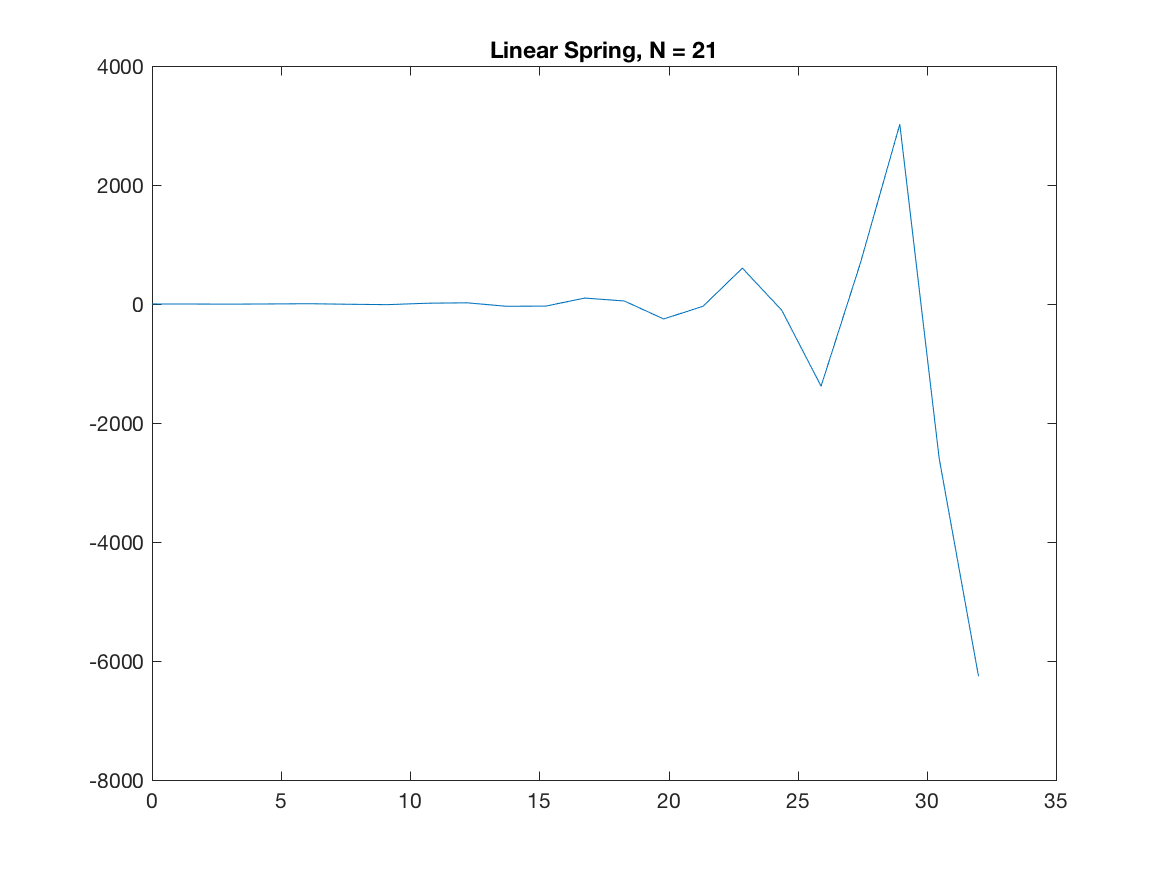
\includegraphics[scale=.4]{Figures/01_01.png}
        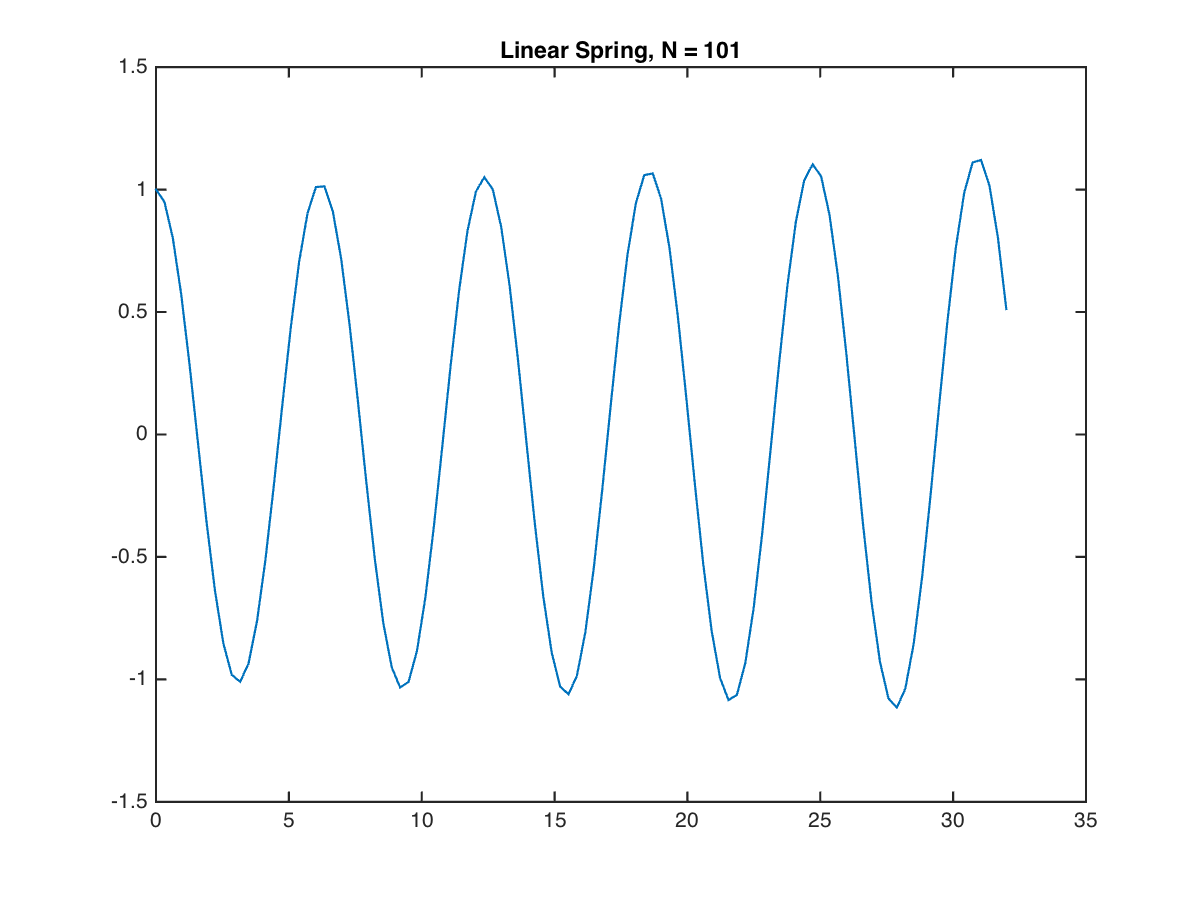
\includegraphics[scale=.4]{Figures/01_02.png}
        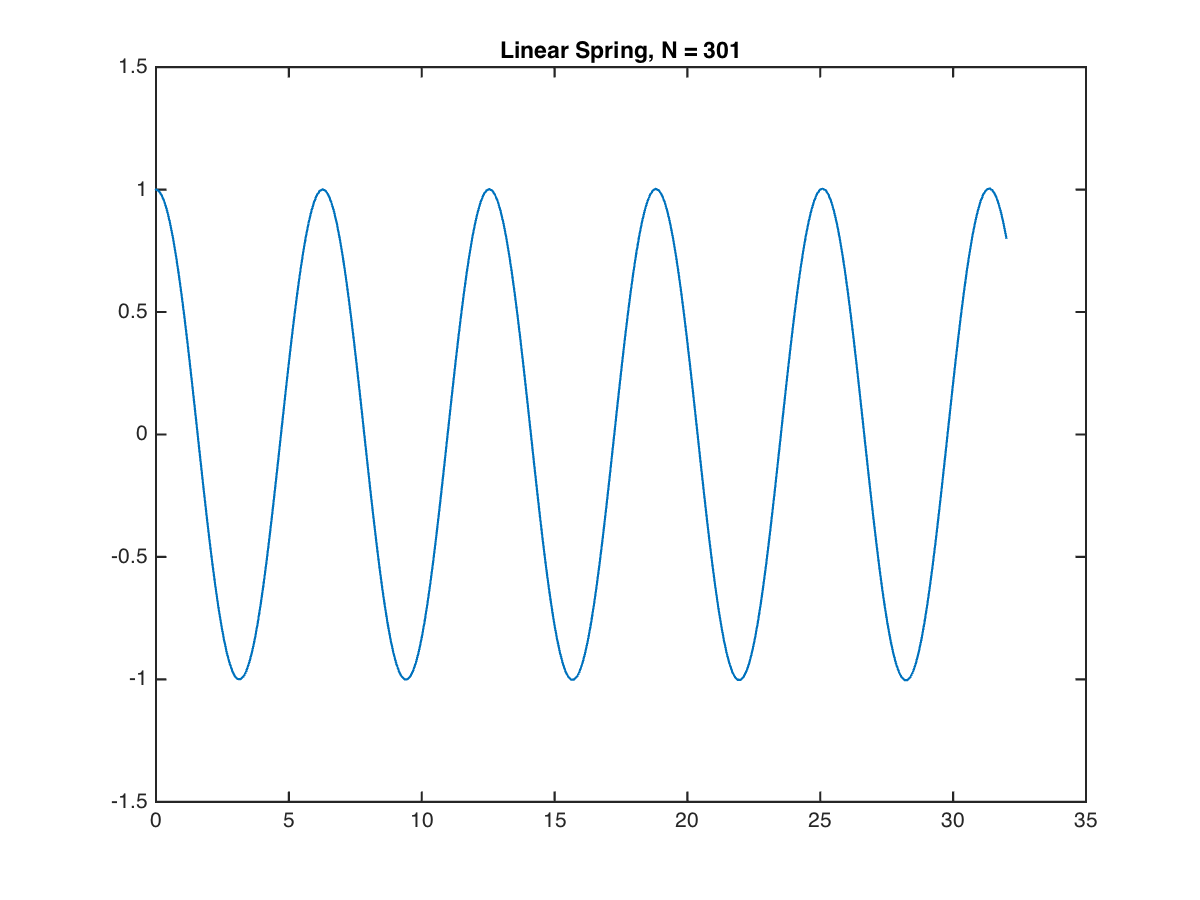
\includegraphics[scale=.4]{Figures/01_03.png}
        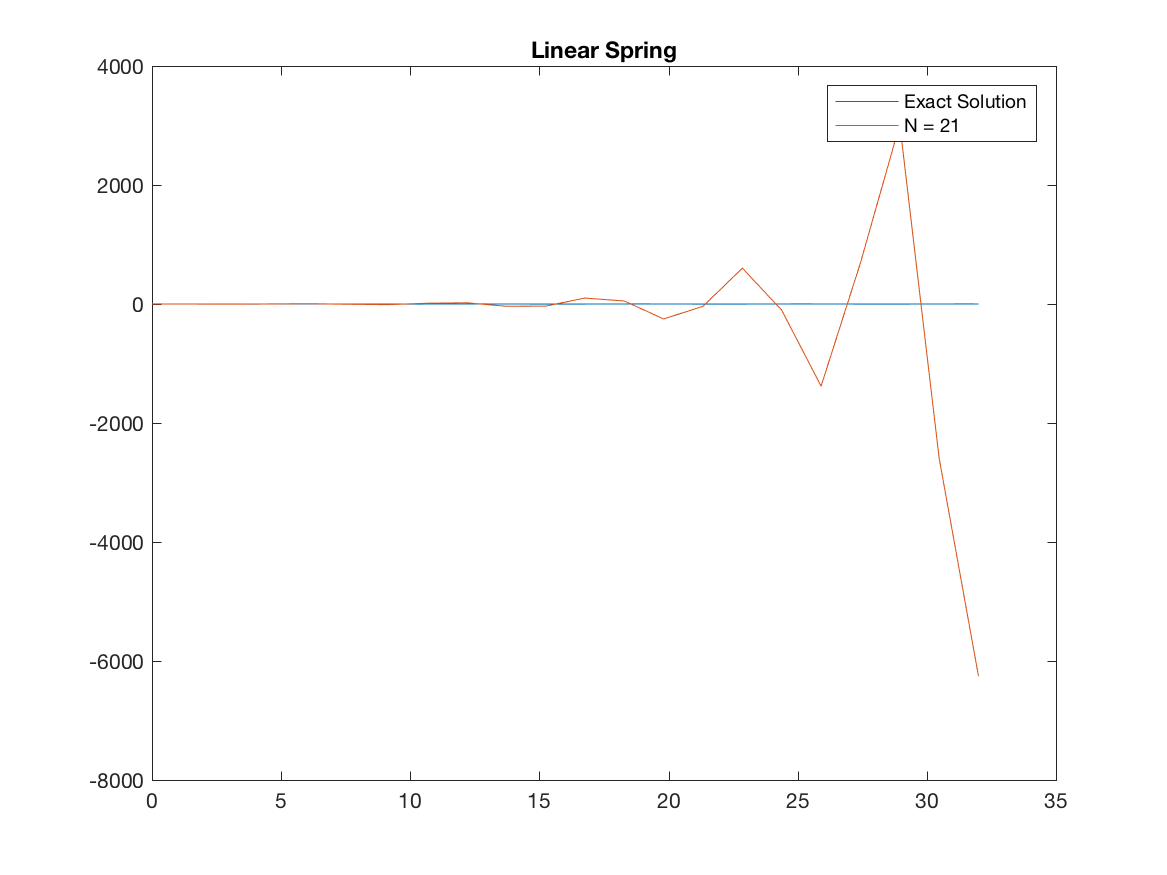
\includegraphics[scale=.4]{Figures/01_04.png}
        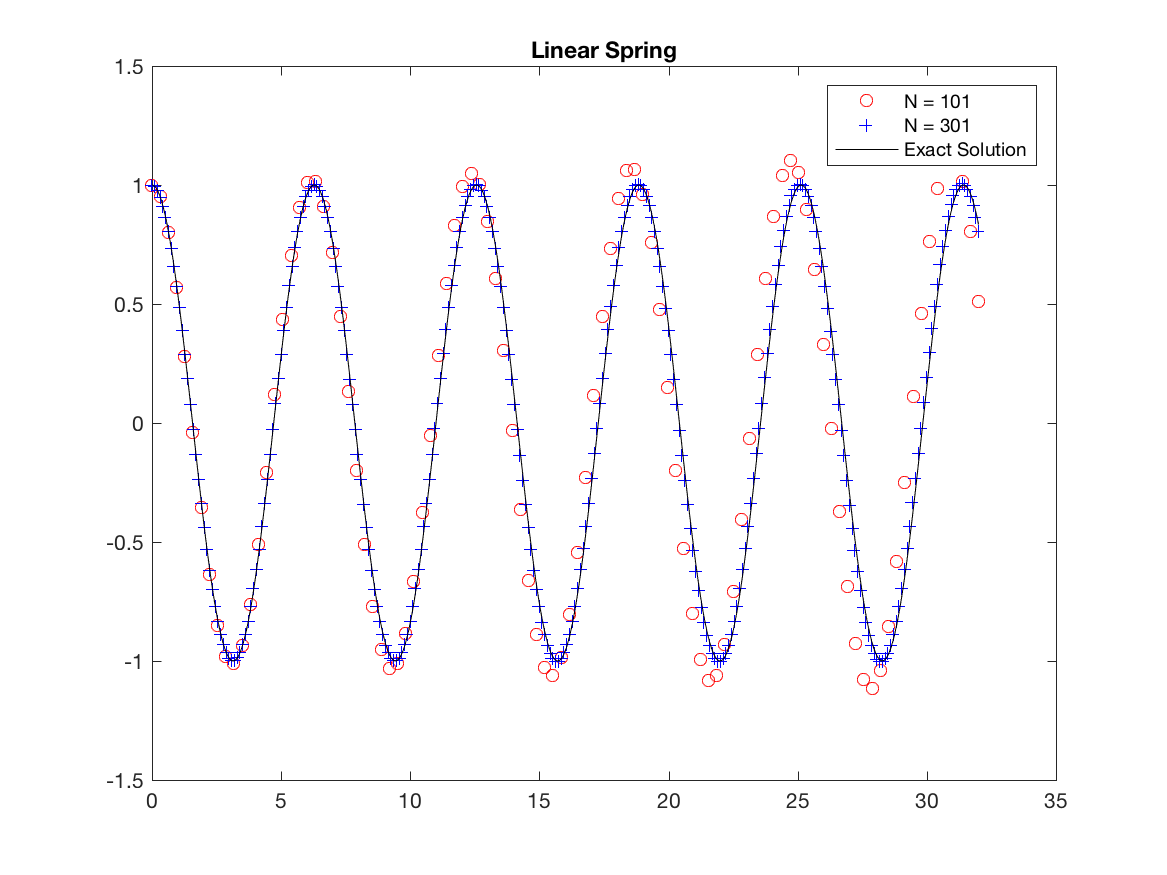
\includegraphics[scale=.7]{Figures/01_05.png}
      \end{center}

      For the damped case, i.e.\ when $\sigma = 0.5$, the following images are
      produced.
      Note that the numerical solution for $N = 21$ doesn't grow rapidly
      and diverge, but is doesn't accurately represent the exact solution.
      Again as $N$ is increased the accuracy of the numerical solution increases.
      \begin{center}
        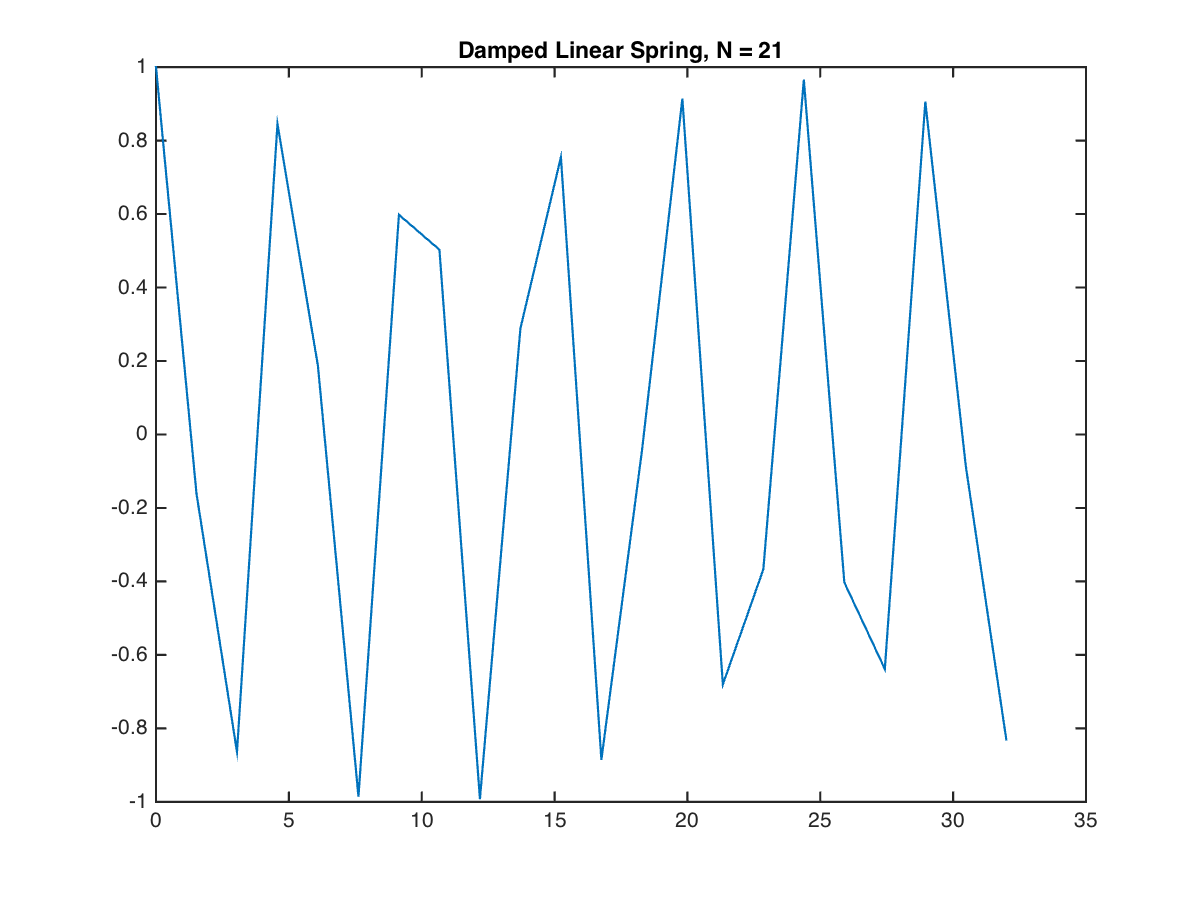
\includegraphics[scale=.4]{Figures/01_06.png}
        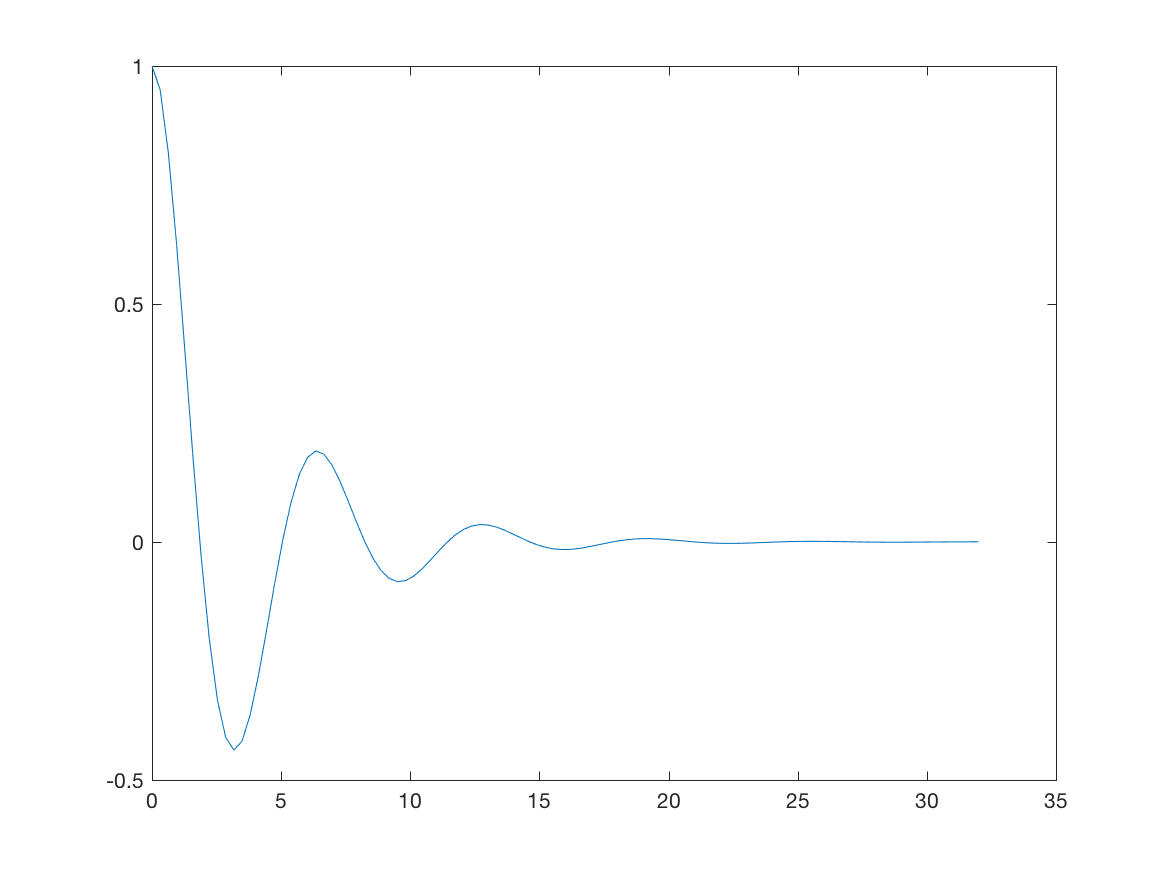
\includegraphics[scale=.4]{Figures/01_07.png}
        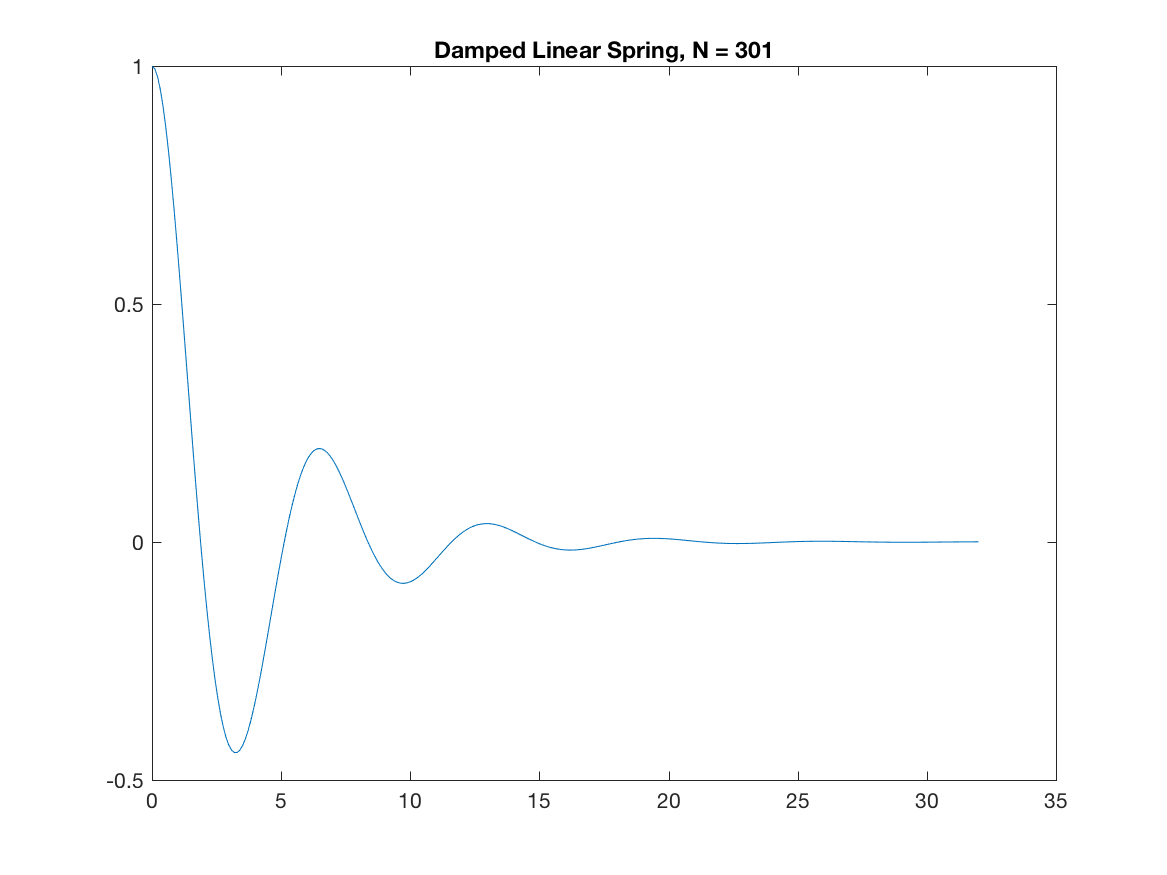
\includegraphics[scale=.4]{Figures/01_08.png}
        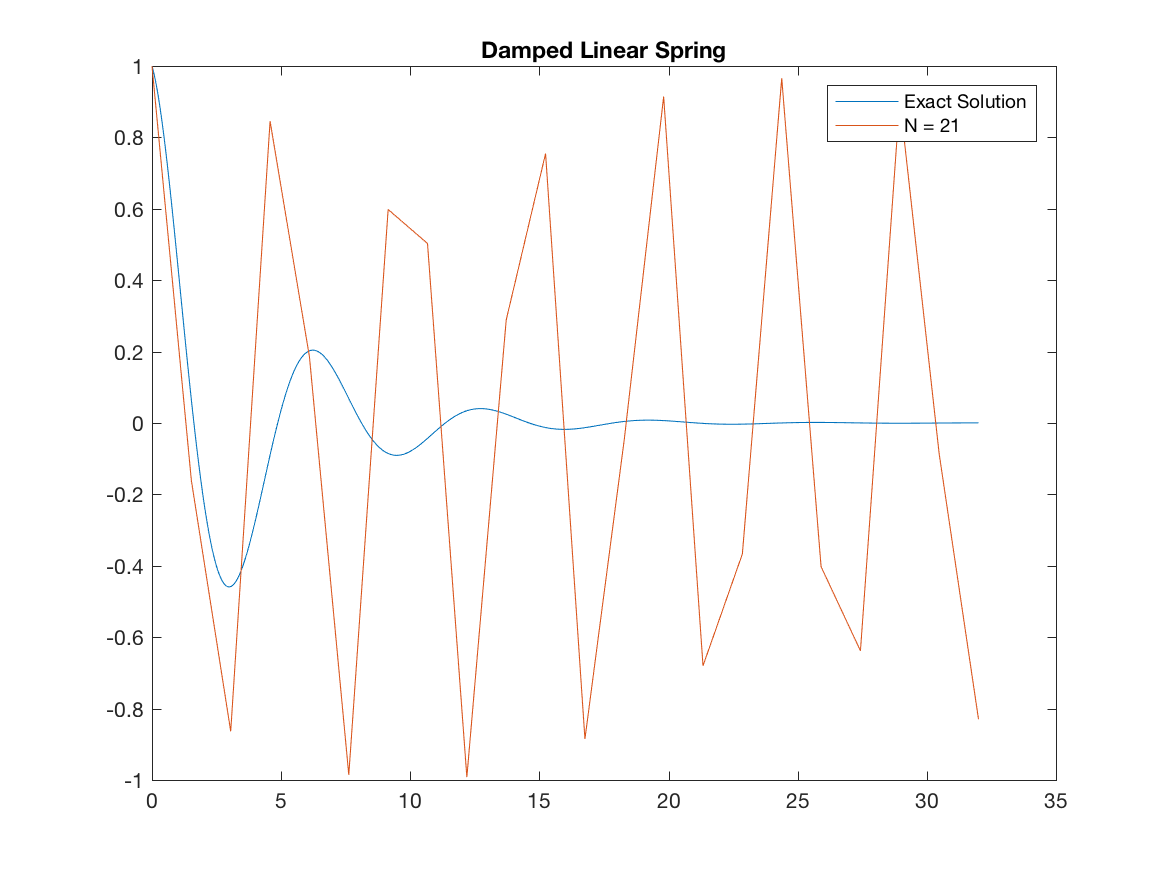
\includegraphics[scale=.4]{Figures/01_09.png}
        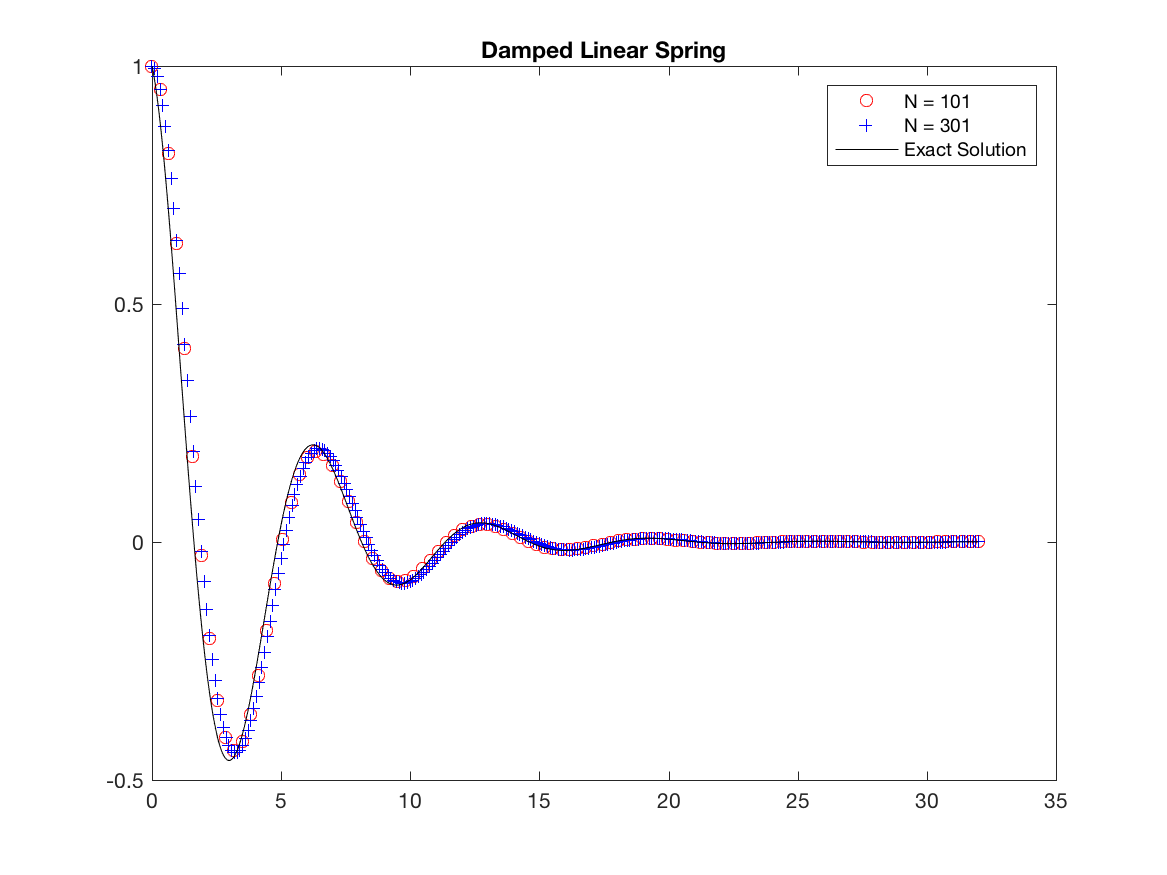
\includegraphics[scale=.7]{Figures/01_10.png}
      \end{center}

    \item[(b)] % Done
      The equation for a nonlinear spring (without damping) is
      \[
        \ddot{Y} + Y - BY^3 = 0.
      \]
      Solve by RK2 out to $t = 32$ with the intial conditions $Y(0) = 1$ and
      $\dot{Y}(0) = 0$.
      Plot $Y(t)$ for $B = 0.2, 0.6, 0.9, 0.999$.
      Chose $N$ large enough to get an accurate solution; that will depend on
      the value of $B$.

      First in order to apply RK2 to this problem we must turn this second order
      ODE into a system of first order ODEs.
      In order to accomplish this let $\dot{Y} = Z$, then we have the following
      system
      \begin{align*}
        \dot{Y} &= Z \\
        \dot{Z} &= -Y - BY^3
      \end{align*}

      The following script now uses the same RK2 method shown in part (a), but with the RHS given
      above.
      \lstinputlisting[language=MATLAB, firstline=75, lastline=108]{H01.m}
      In this script I used $N = 1000$ for $B = 0.2, 0.6, 0.9$ and $N = 3000$ for
      $B = .999$.
      $B$ is controlling the nonlinearity of the spring and the larger that
      contribution is the smaller the timestep needs to be.
      The following images are produced.
      \begin{center}
        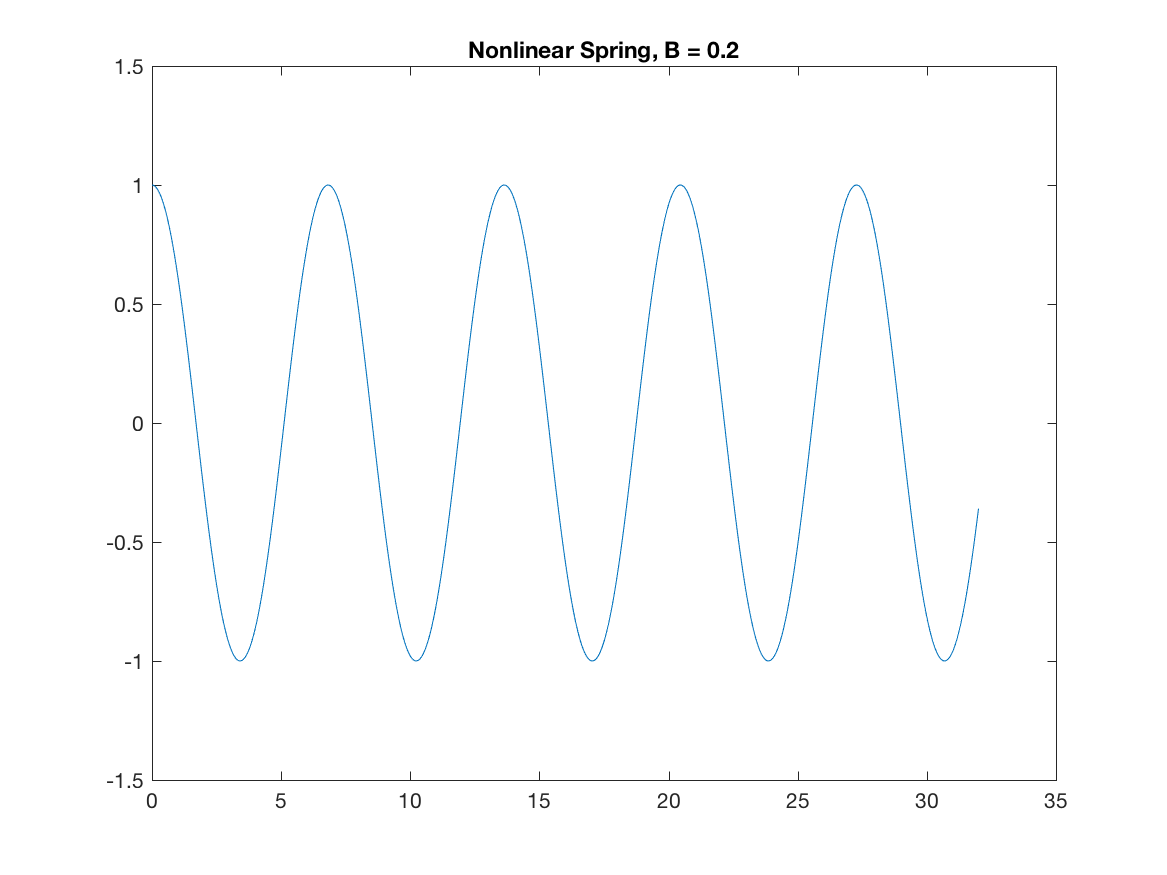
\includegraphics[scale=.4]{Figures/01_11.png}
        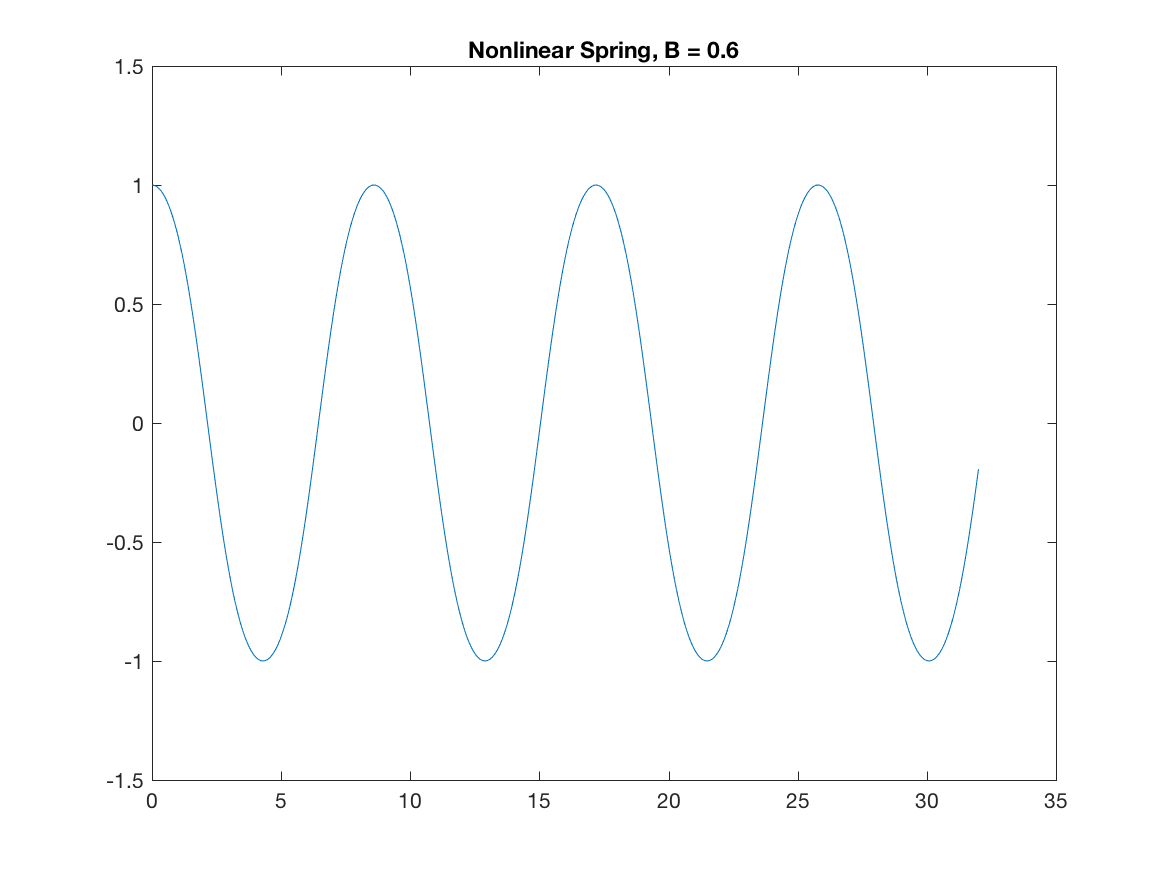
\includegraphics[scale=.4]{Figures/01_12.png}
        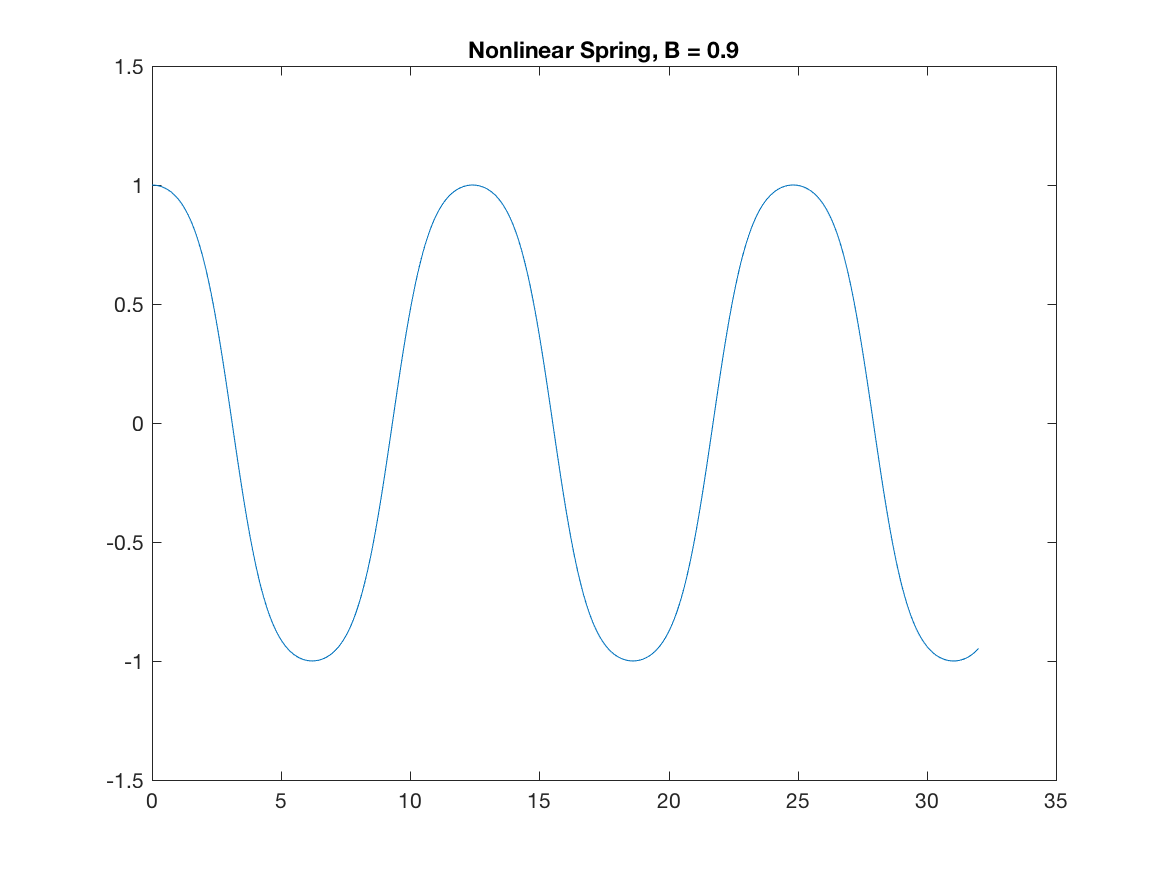
\includegraphics[scale=.4]{Figures/01_13.png}
        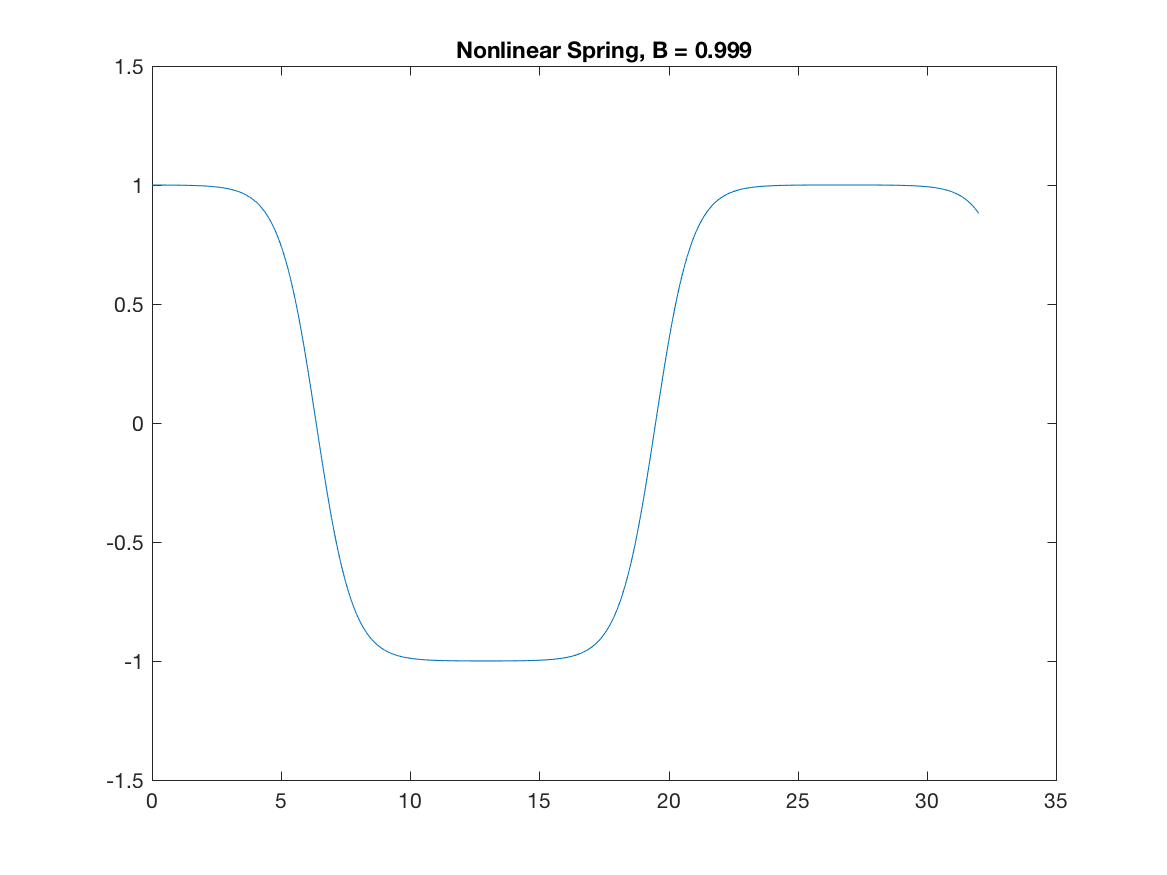
\includegraphics[scale=.4]{Figures/01_14.png}
      \end{center}

  \item[\#3]
    Repeat the linear spring computation (ex. 2.a) with AB2.
    What does the solution for $\sigma=0.0$ tell you about the stability of AB2?

    I implemented the following function to run AB2 method for any RHS function.
    \lstinputlisting[language=MATLAB]{AB2.m}
    The following script now repeats exercise 2.a with this function instead of RK2.
    \lstinputlisting[language=MATLAB, firstline=110]{H01.m}

    The following images were produced in the undamped case.
    Note that for $N = 21$ the solution diverges rapidly, much more rapidly
    than for RK2.
    This shows that adams-bashforth has a smaller area of stability as the time
    step needs to be much smaller in order to get an accurate solution.
    However for $N = 101$ and $N = 301$ the solutions are relatively accurate if
    less so than for RK2.
    \begin{center}
      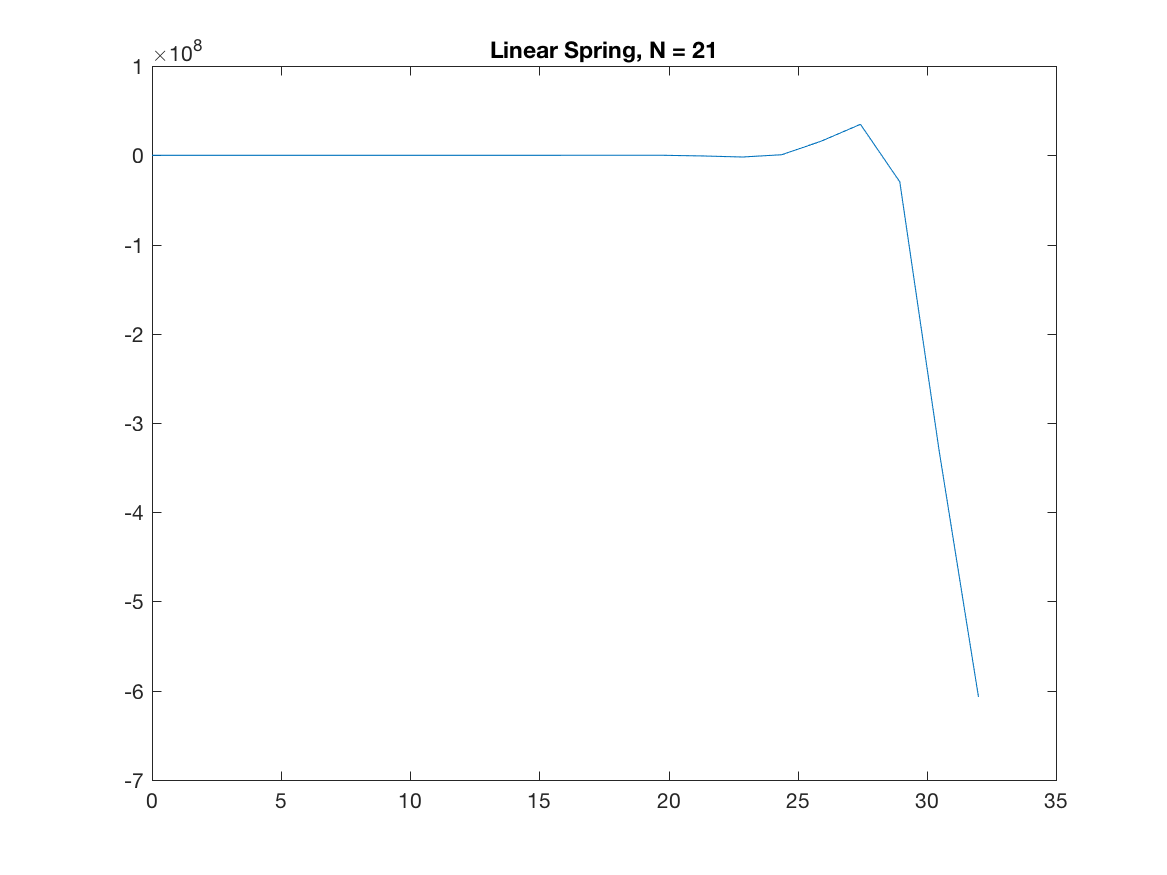
\includegraphics[scale=.4]{Figures/01_15.png}
      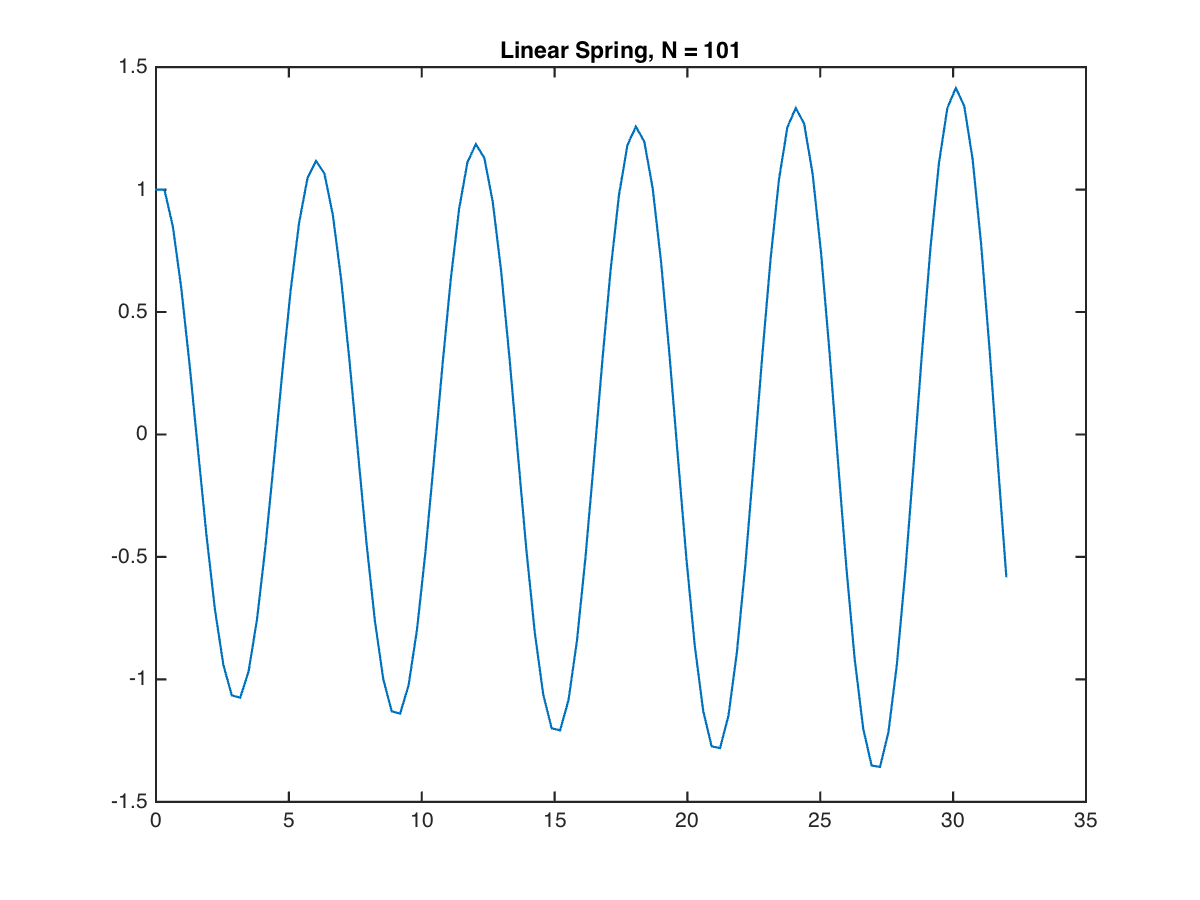
\includegraphics[scale=.4]{Figures/01_16.png}
      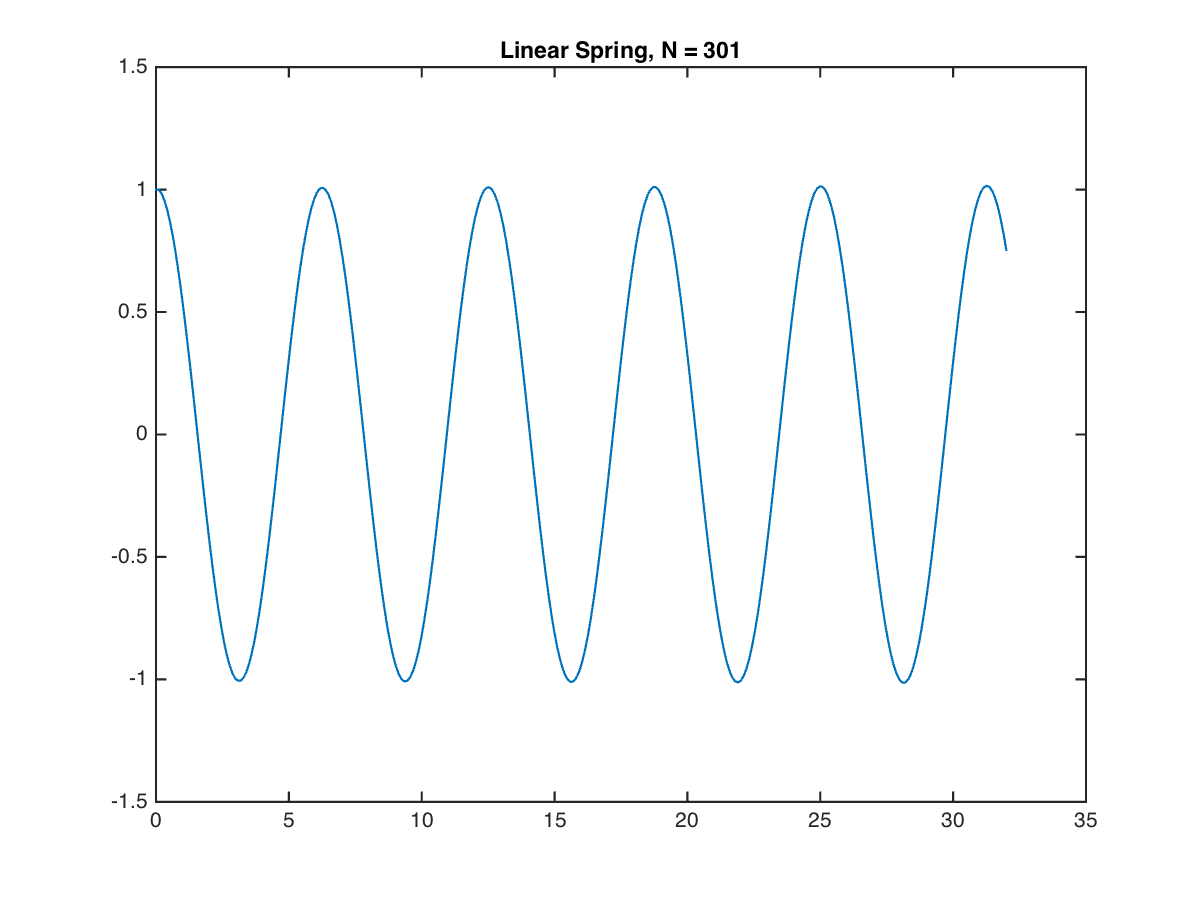
\includegraphics[scale=.4]{Figures/01_17.png}
      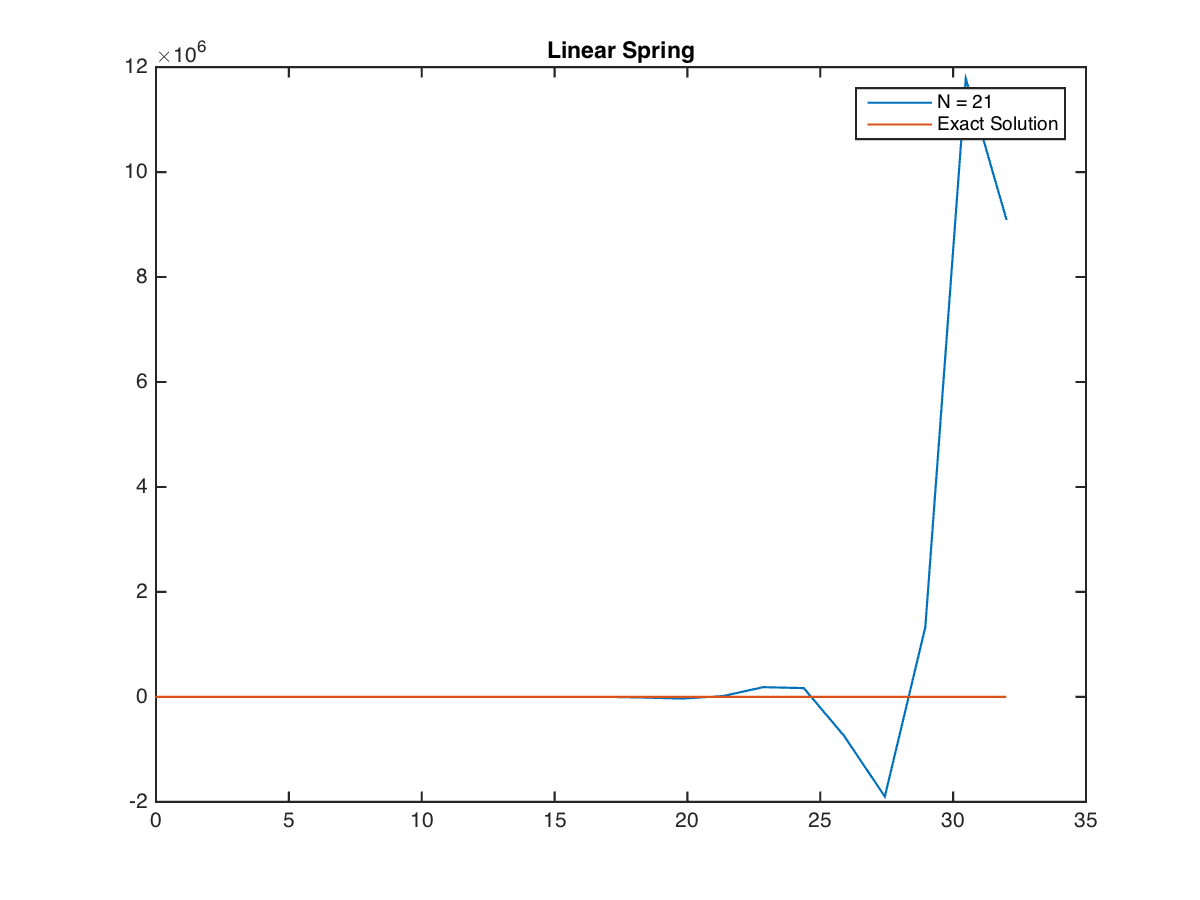
\includegraphics[scale=.4]{Figures/01_18.png}
      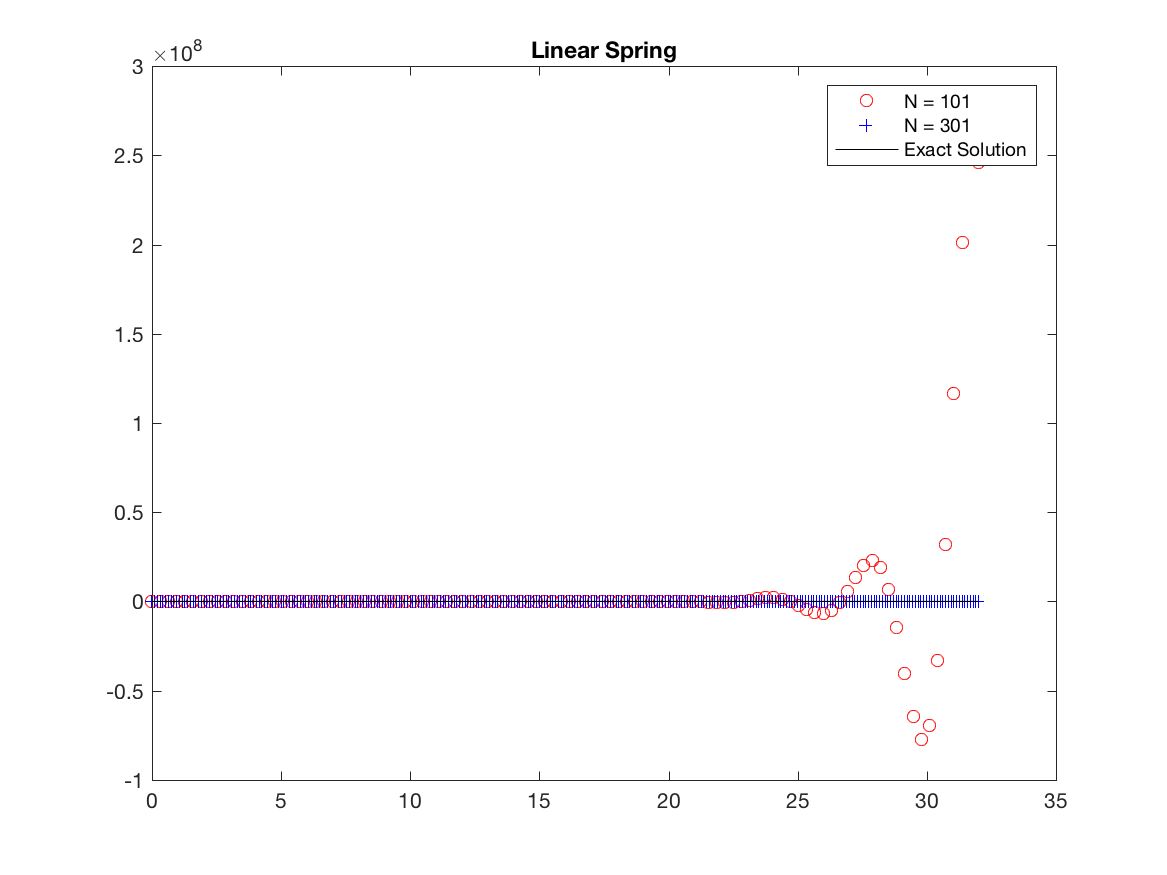
\includegraphics[scale=.7]{Figures/01_19.png}
    \end{center}

    The following images were produced for the damped case
    Note that the solution diverges for $N = 21$.
    \begin{center}
      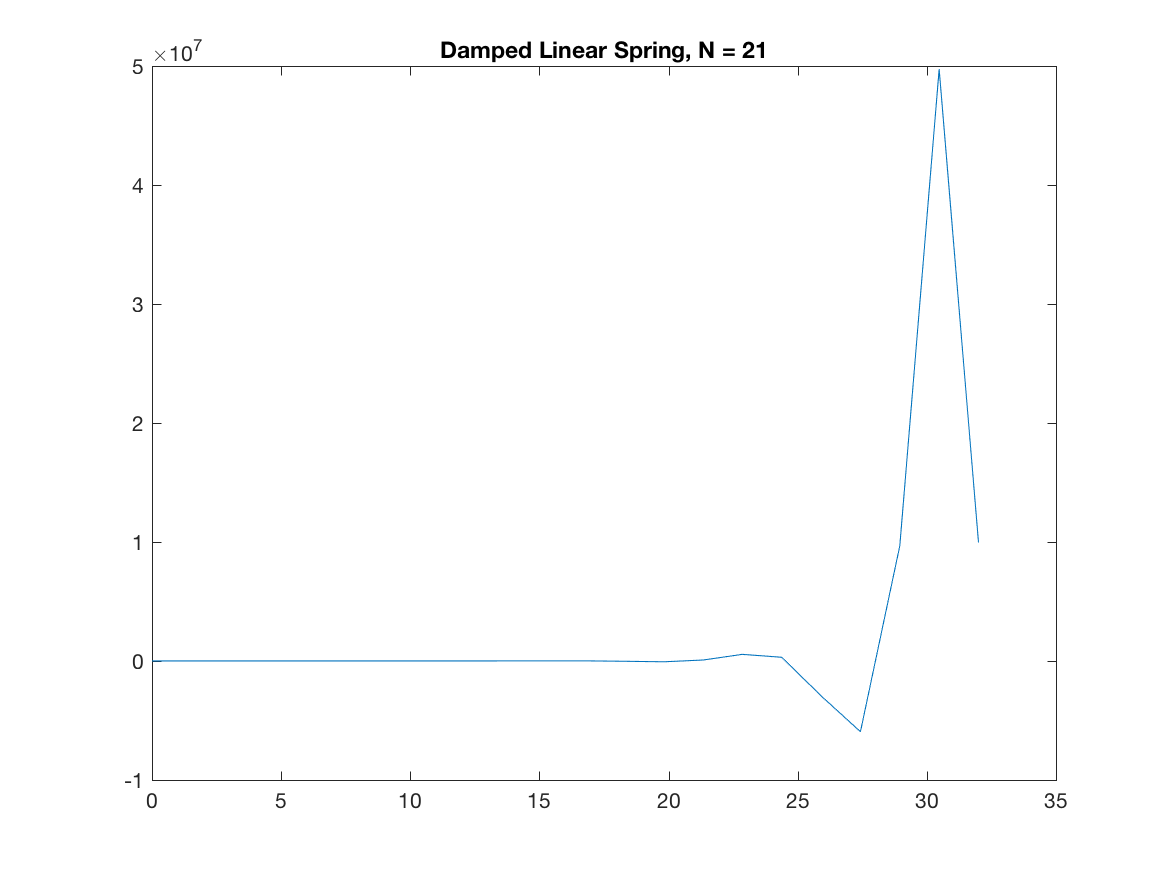
\includegraphics[scale=.4]{Figures/01_20.png}
      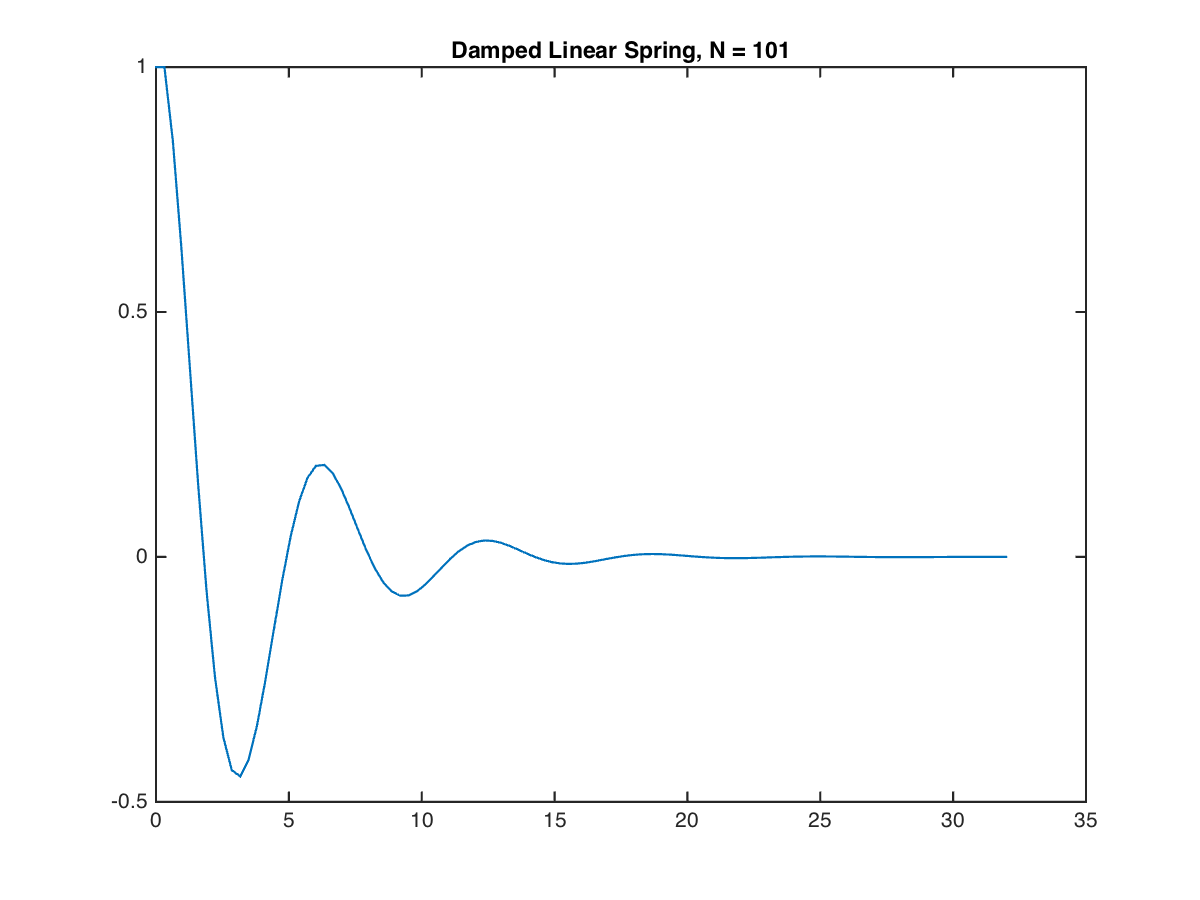
\includegraphics[scale=.4]{Figures/01_21.png}
      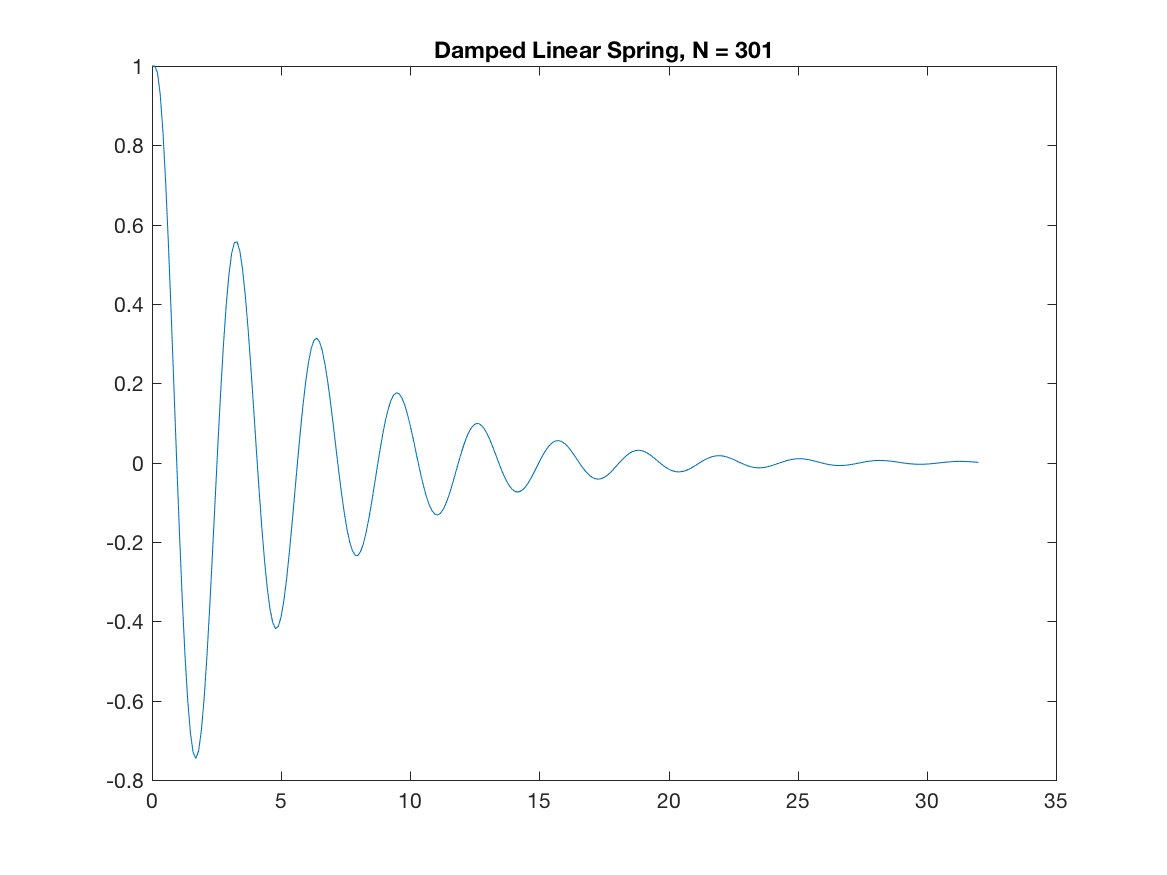
\includegraphics[scale=.4]{Figures/01_22.png}
      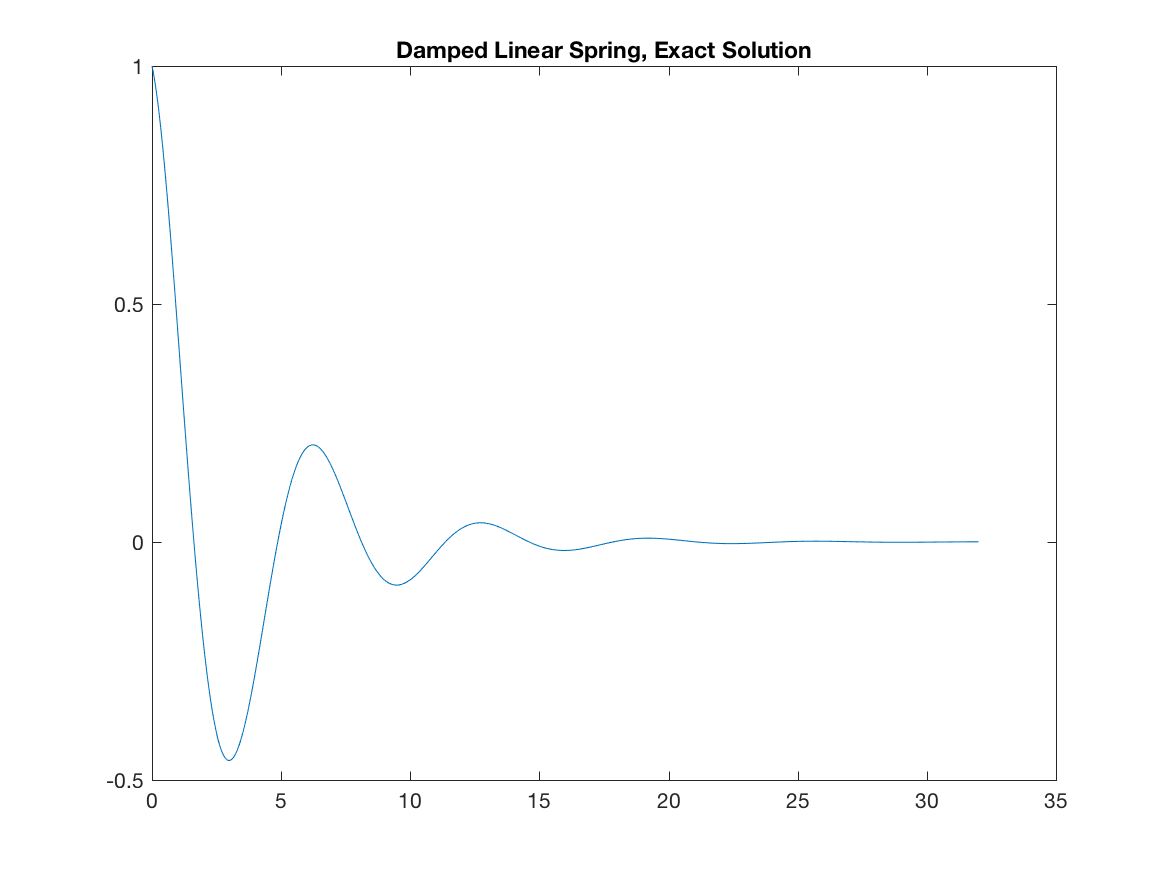
\includegraphics[scale=.4]{Figures/01_23.png}
      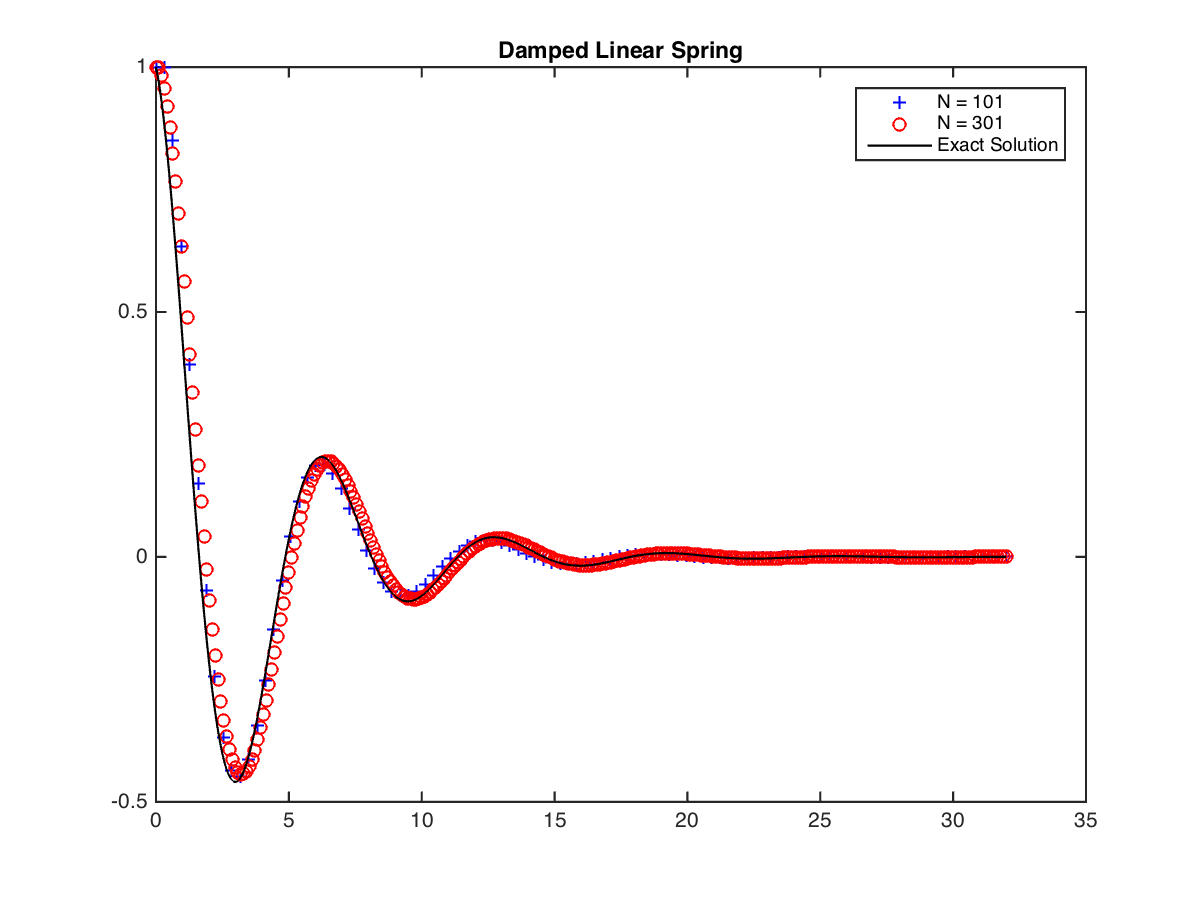
\includegraphics[scale=.7]{Figures/01_24.png}
    \end{center}
\end{enumerate}
\end{document}
